\subsection[E]{Energia Meccanica}
        \begin{frame}{E vs T | 100, 500, 2500 anni}
            \begin{columns}
                \column{.5\textwidth}
                    \centering        
                    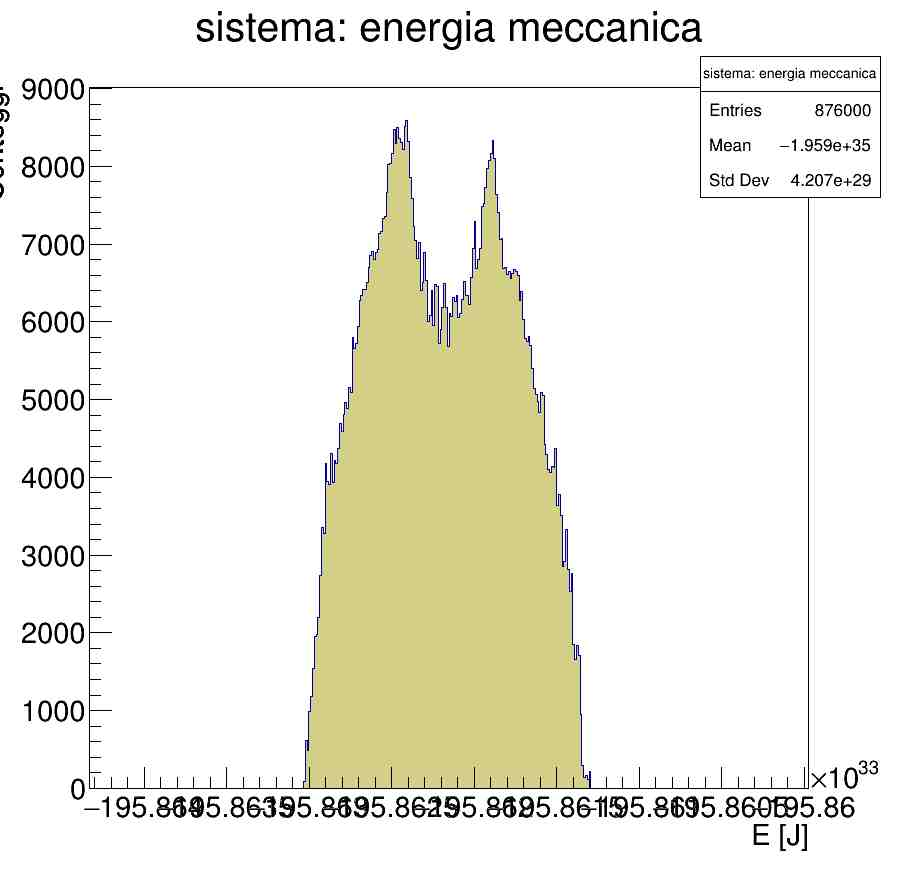
\includegraphics[width=5cm,height=3.75cm]{4_energia/E_100_3600.jpg}\\
                    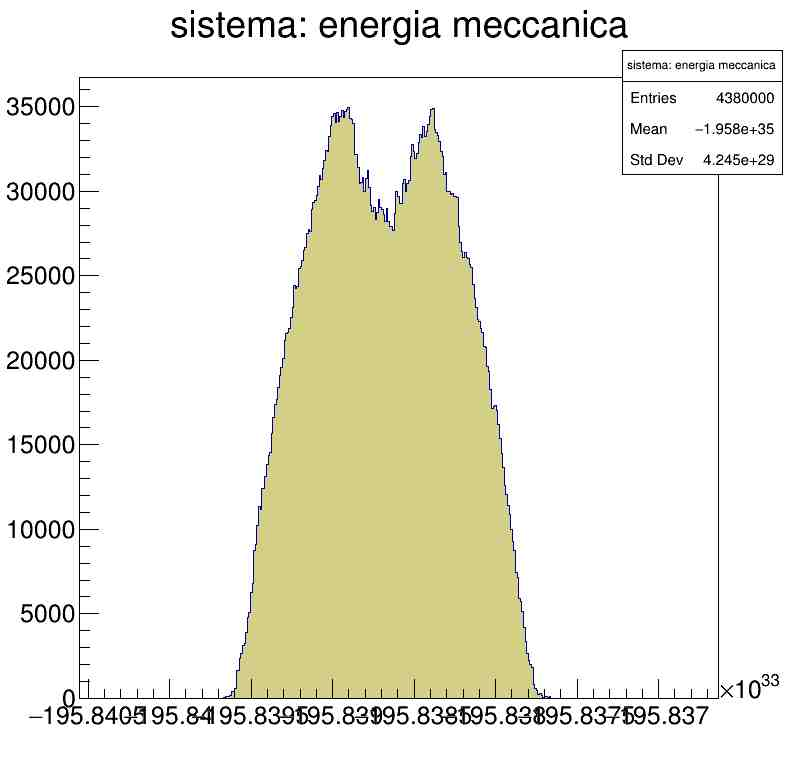
\includegraphics[width=5cm,height=3.75cm]{4_energia/E_500_3600.jpg}
                    \label{cfr::ET}              
                \column{.5\textwidth}
                    \centering        
                    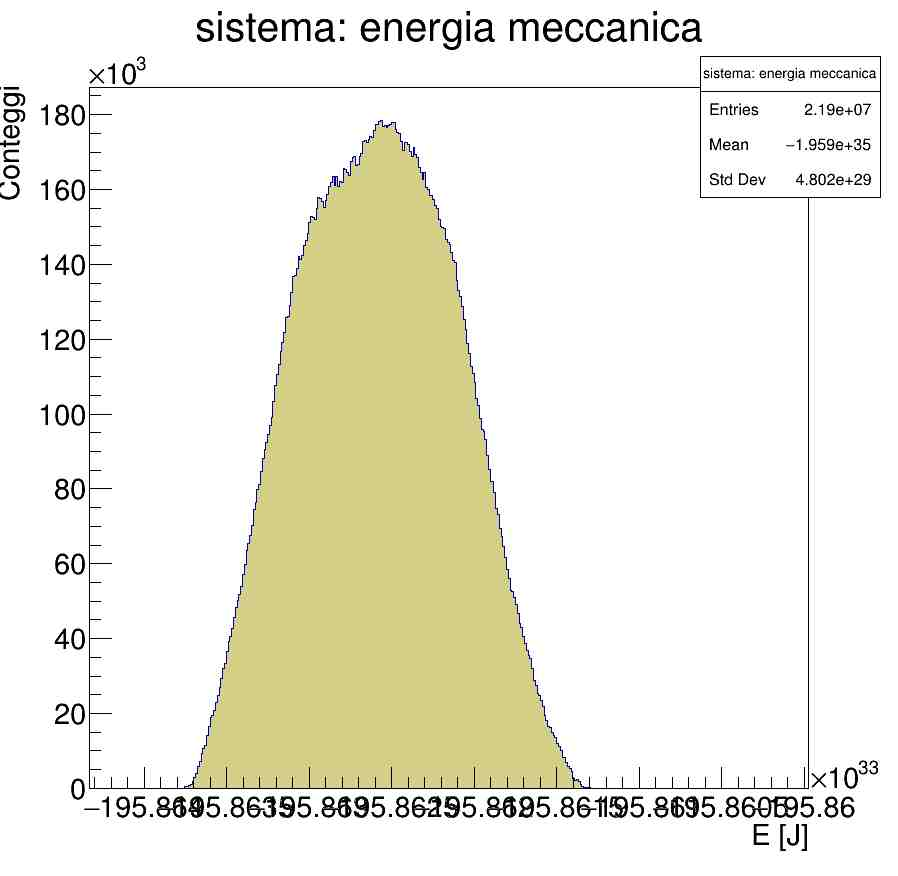
\includegraphics[width=5cm,height=3.75cm]{4_energia/E_2500_3600_stretto.jpg}\\
                    \label{cfr::ET1}
                    Media vicina - leggero aumento della DevStd col tempo
            \end{columns}
        \end{frame}
        \begin{frame}{E vs deltaT | 60, 1800, 3600 secondi}
            \begin{columns}
                \column{.5\textwidth}
                    \centering        
                    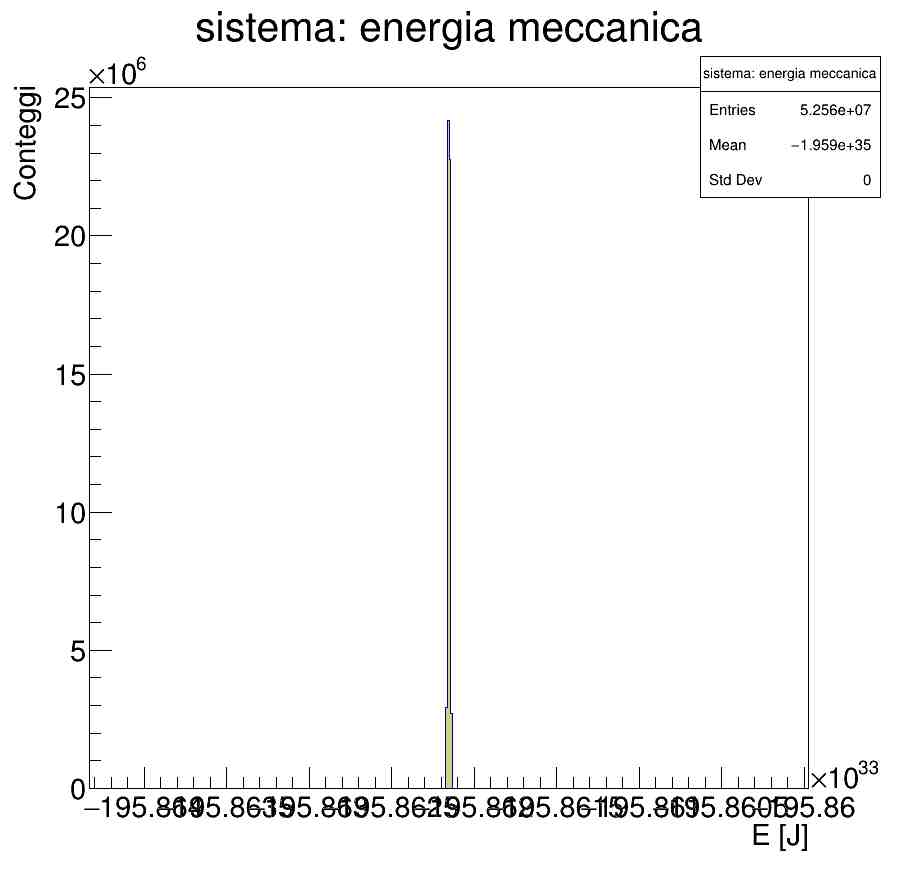
\includegraphics[width=5cm,height=3.75cm]{4_energia/E_100_60.jpg}\\
                    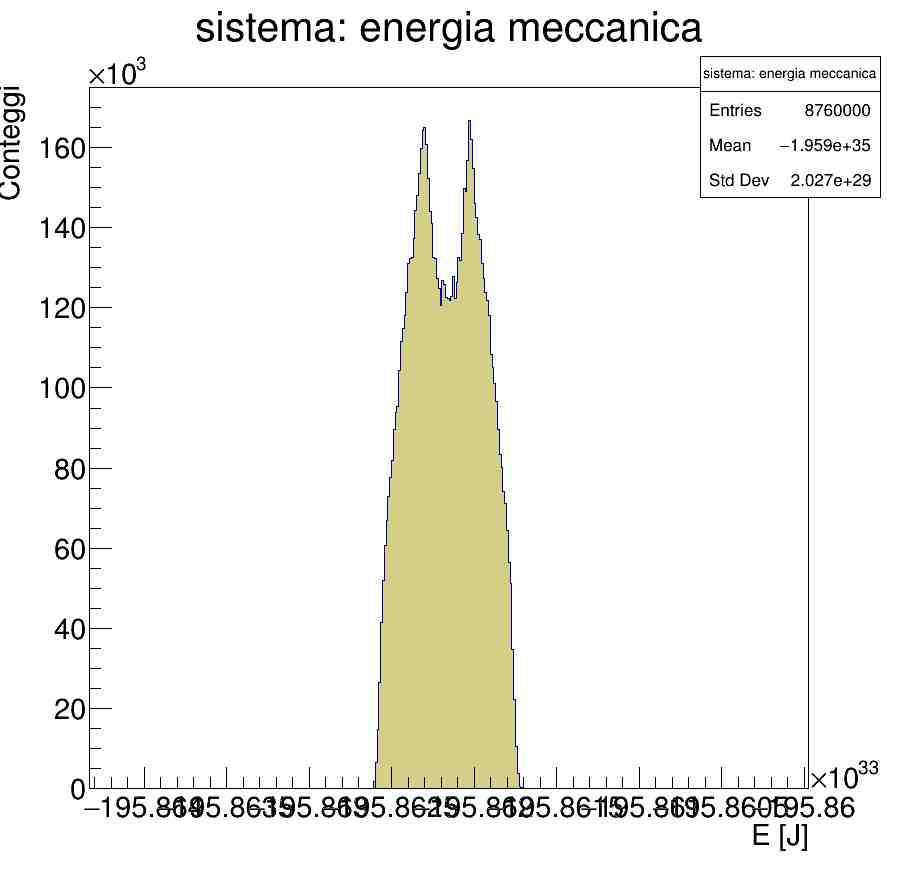
\includegraphics[width=5cm,height=3.75cm]{4_energia/E_500_1800.jpg}
                    \label{cfr::E3}              
                \column{.5\textwidth}
                    \centering        
                    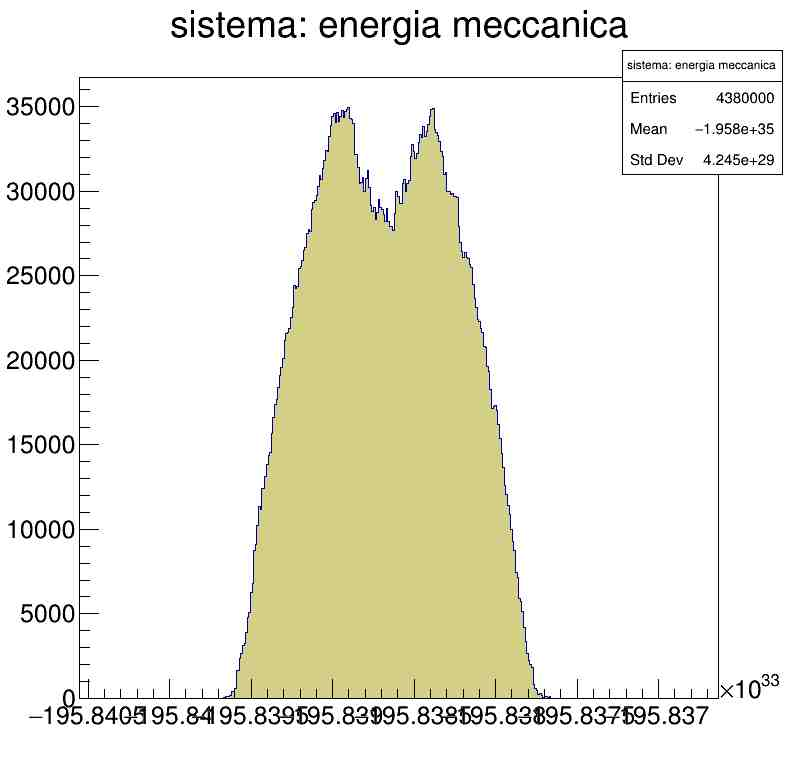
\includegraphics[width=5cm,height=3.75cm]{4_energia/E_500_3600.jpg}\\
                    \label{cfr::E2T}
                    Si nota molto di più l'effetto rispetto agli istogrammi di L
            \end{columns}            
        \end{frame}
        \begin{frame}{E vs posizioni iniziali | perielio, afelio, medie, miste}
            \begin{columns}
                \column{.5\textwidth}
                    \centering        
                    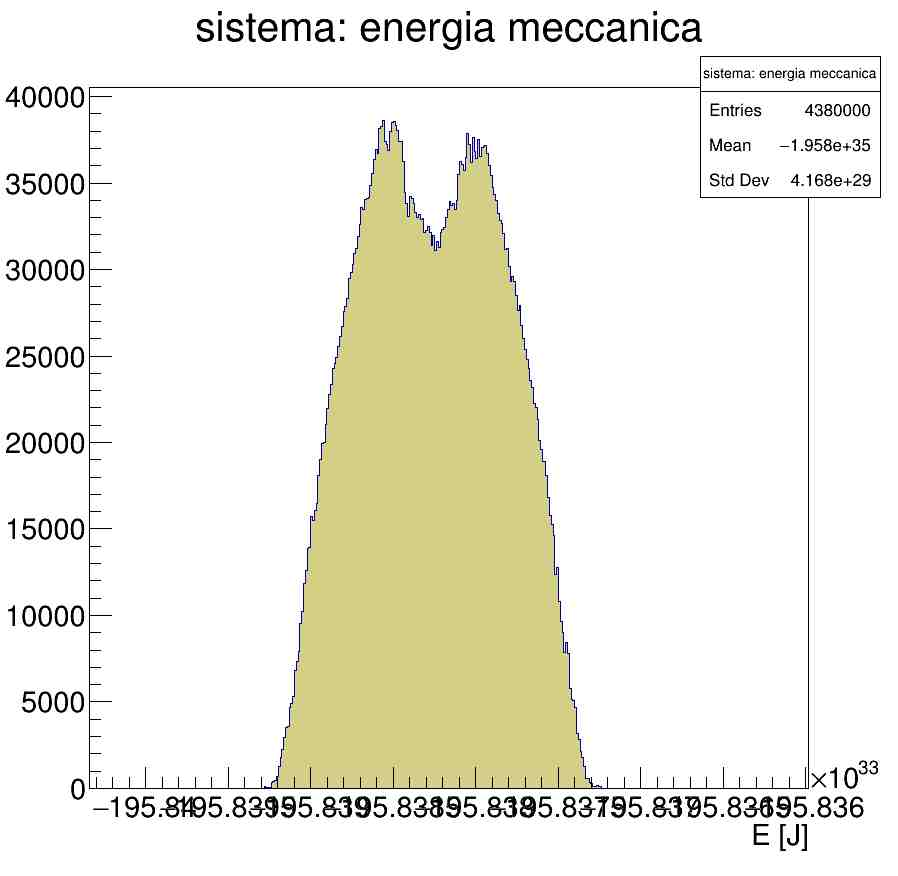
\includegraphics[width=5cm,height=3.75cm]{4_energia/E_500_peri.jpg}\\
                    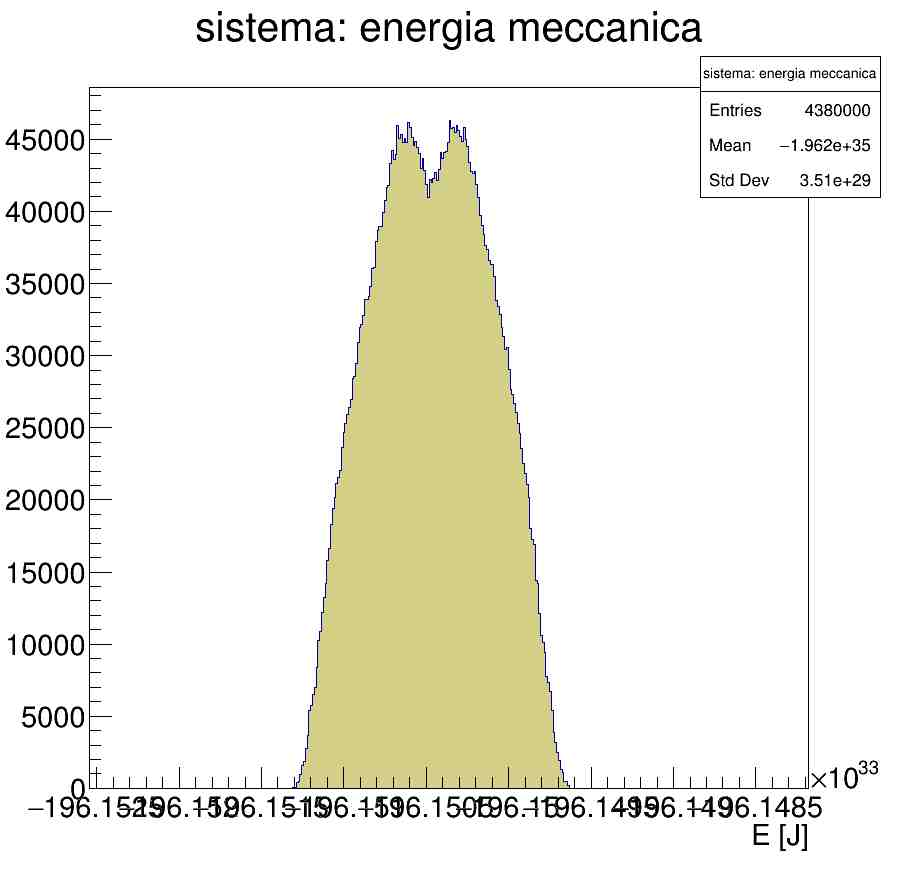
\includegraphics[width=5cm,height=3.75cm]{4_energia/E_500_afe.jpg}
                    \label{cfr::E4T}              
                \column{.5\textwidth}
                    \centering        
                    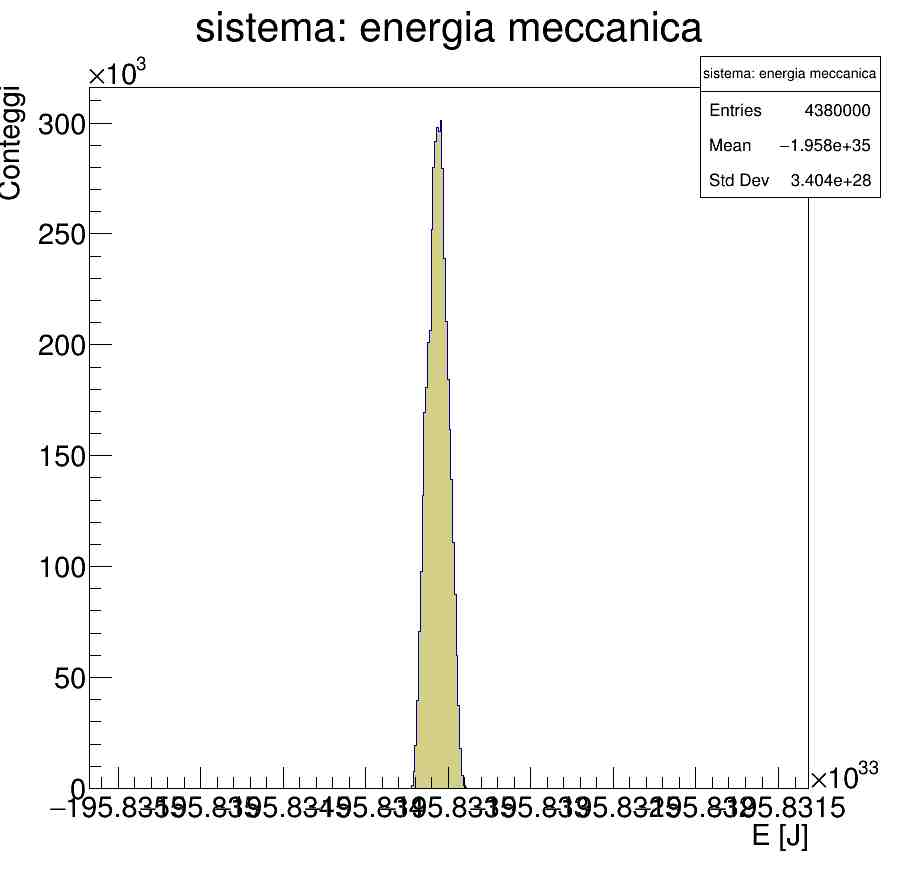
\includegraphics[width=5cm,height=3.75cm]{4_energia/E_500_medi.jpg}\\
                    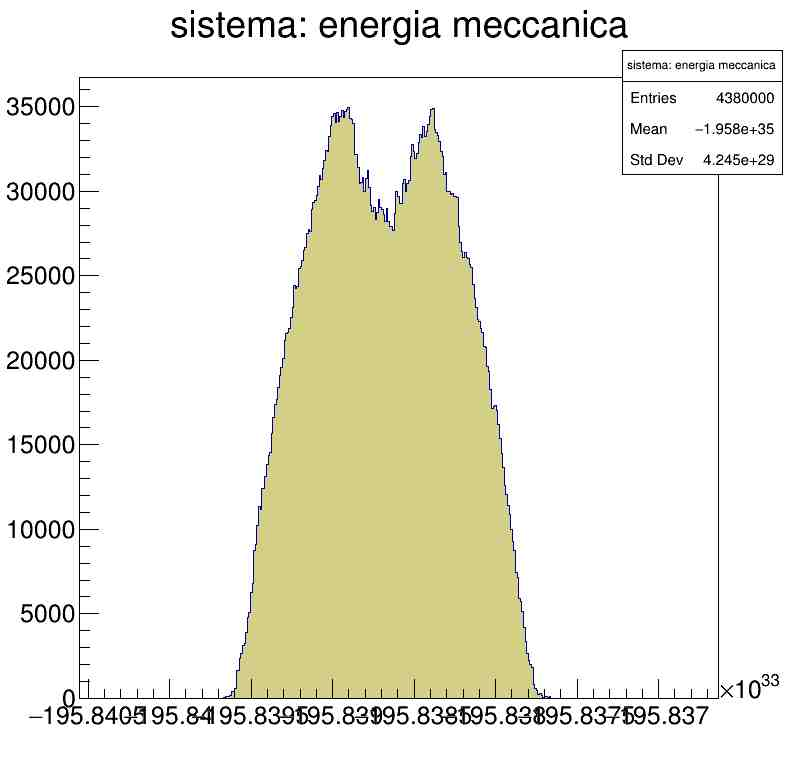
\includegraphics[width=5cm,height=3.75cm]{4_energia/E_500_3600.jpg}
                    \label{cfr::E6T}      
            \end{columns}
        \end{frame}

        \begin{frame}{Istogramma con Python}
            \begin{figure}
                \centering
                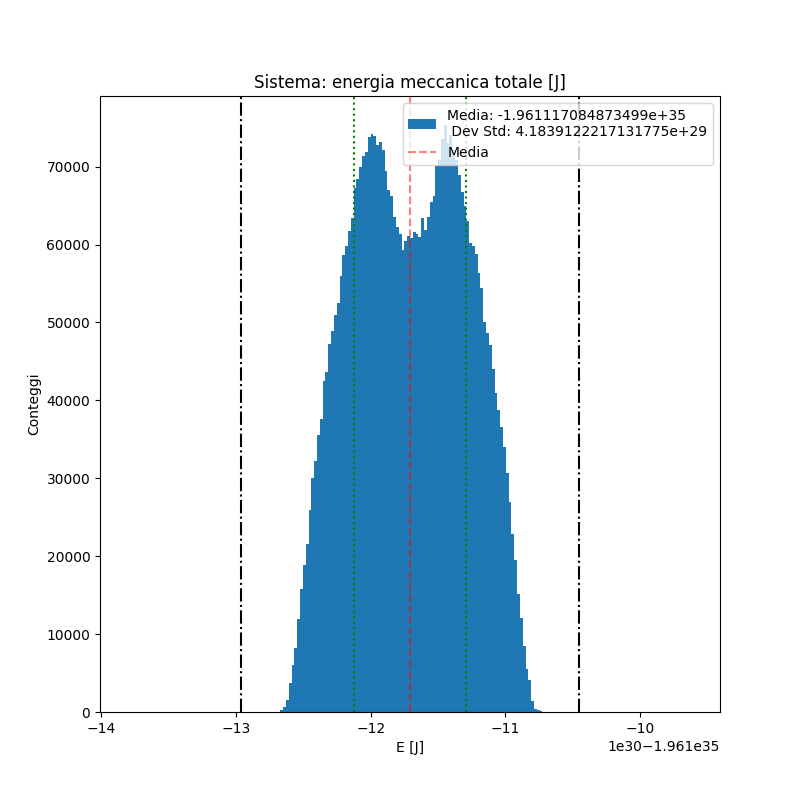
\includegraphics[height=8cm]{4_energia/E_500_3600_py-.png}
                %\caption{Caption}
                %\label{fig:enter-label}
            \end{figure}
        \end{frame}

        \subsubsection[DP]{Double Peak}
                    \begin{frame}{Studio del doppio picco}
            \begin{columns}
                \column{.5\textwidth}
                    \centering        
                    \includegraphics[width=5cm,height=3.75cm]{4_energia/peak/}\\
                    %quì cinetica vs Pot
                    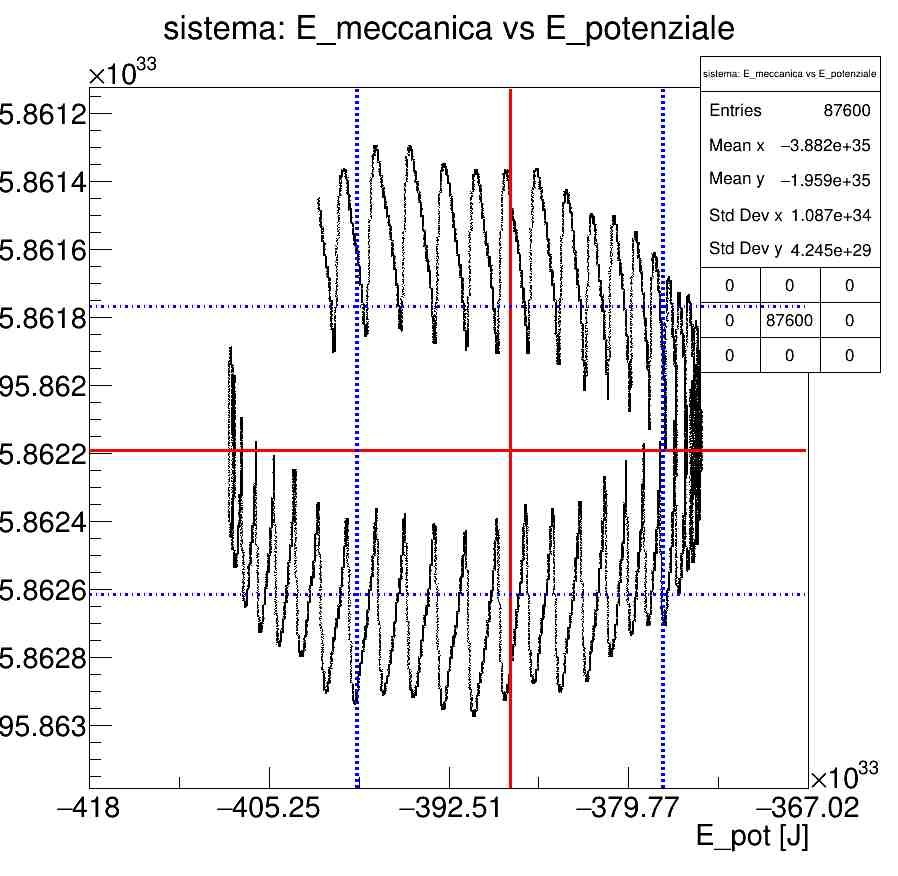
\includegraphics[width=5cm,height=3.75cm]{4_energia/peak/Mec_pot.jpg}
                    \label{cfr::Epc}              
                \column{.5\textwidth}
                    \centering        
                    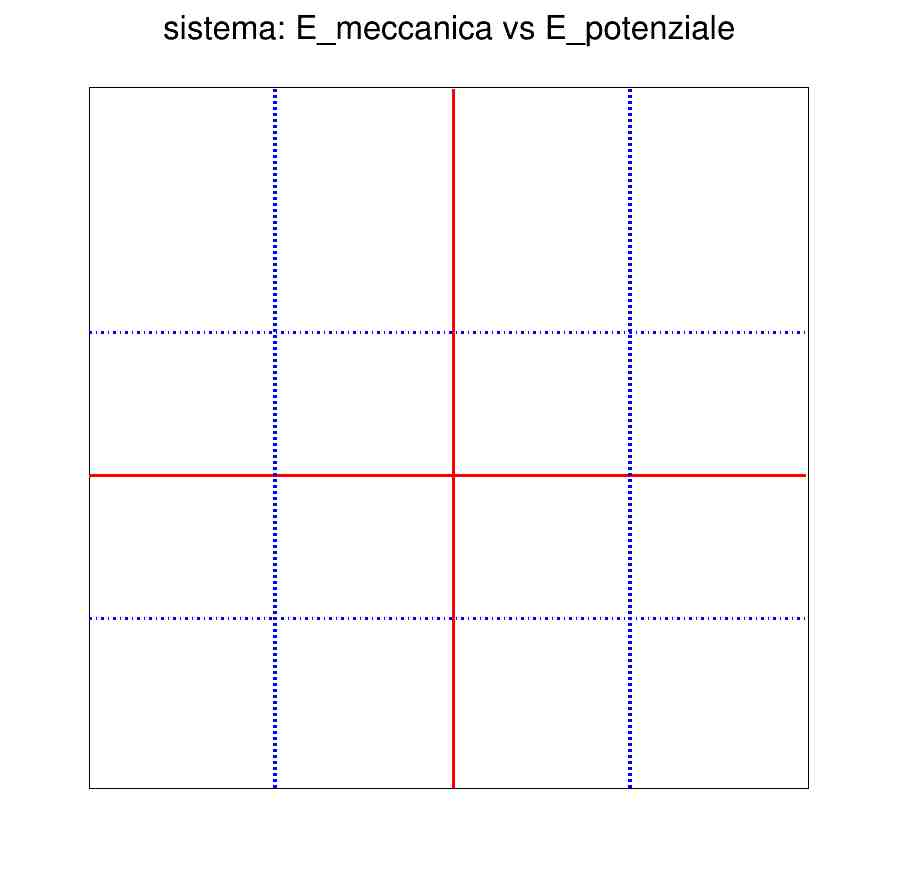
\includegraphics[width=5cm,height=3.75cm]{4_energia/peak/m_p_500.jpg}\\
                    %qui grafico E vs Pot dopo 500a
                    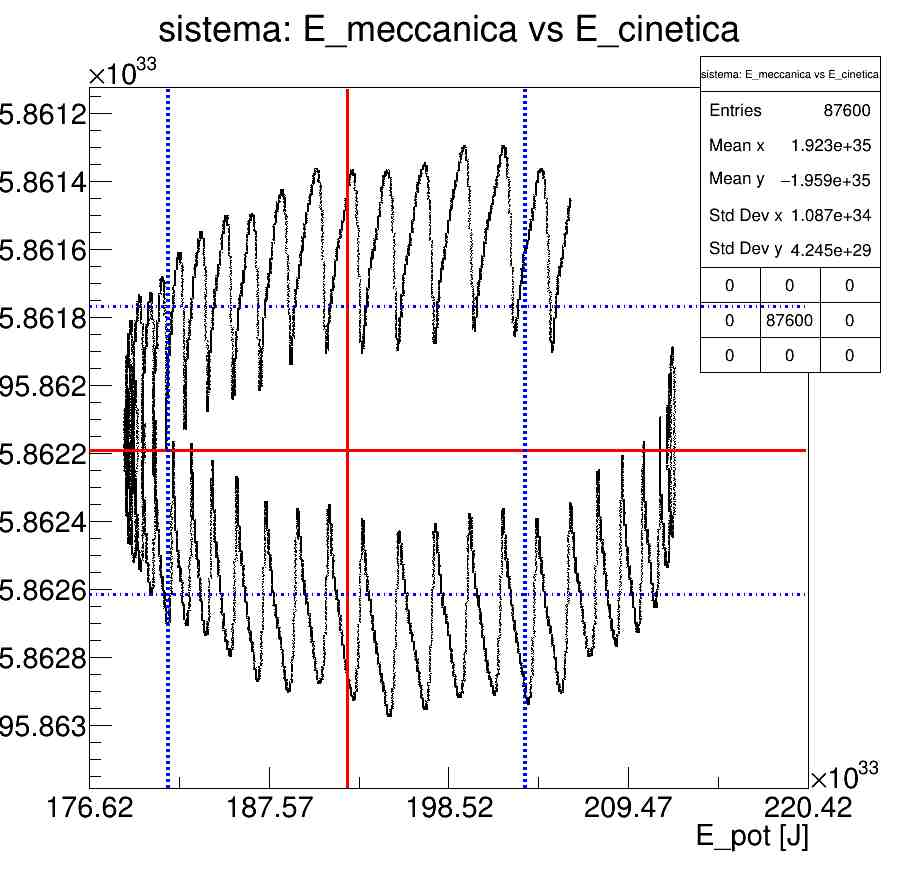
\includegraphics[width=5cm,height=3.75cm]{4_energia/peak/mec_cin.jpg}
                    \label{cfr::eme}      
            \end{columns}
        \end{frame}
        \begin{frame}{Studio del doppio picco}
            \begin{columns}
                \column{.5\textwidth}
                    \centering        
                    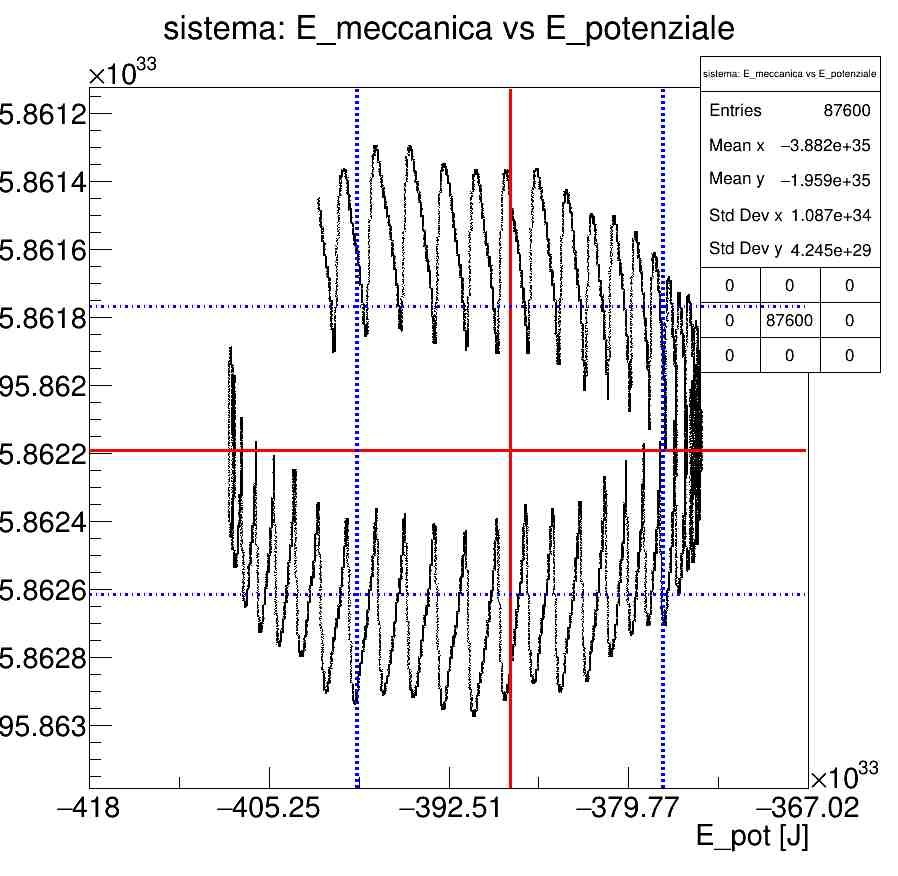
\includegraphics[width=5cm,height=3.75cm]{4_energia/peak/Mec_pot.jpg}\\
                    \label{cfr::E4T}              
                \column{.5\textwidth}
                    \centering        
                    \includegraphics[width=5cm,height=3.75cm]{4_energia/peak/mec_gio.jpg}\\
                    %qui grafico E vs dgiove-sole
                    \label{cfr::E6T}      
            \end{columns}
        \end{frame}

        \begin{frame}{Andamenti nel tempo}
            \begin{figure}
                \centering
                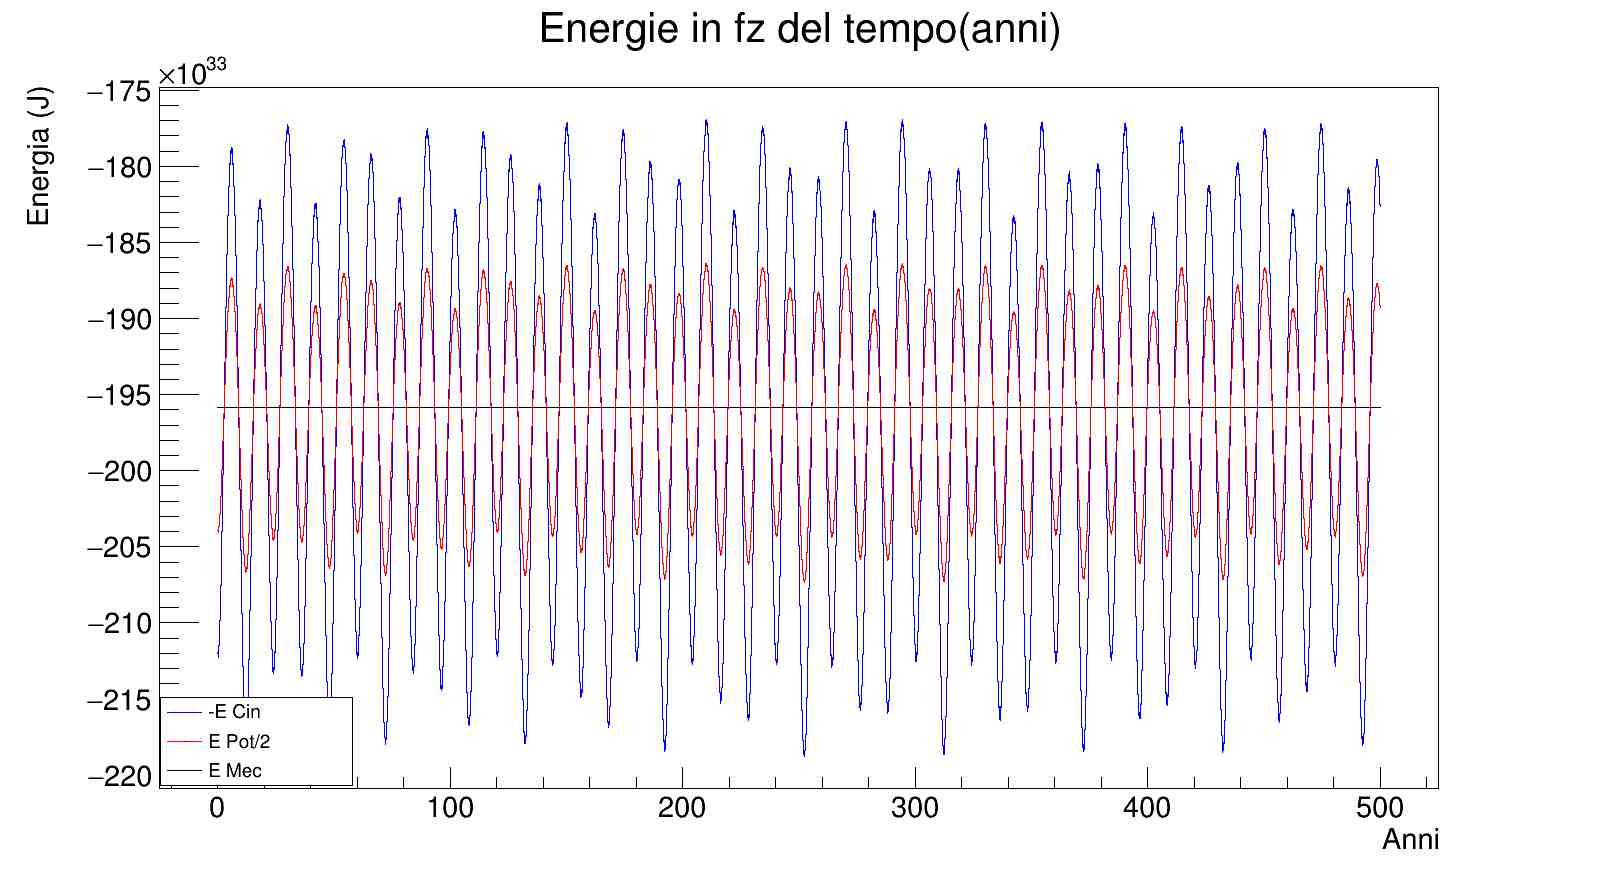
\includegraphics[width=\textwidth]{4_energia/peak/E_tempo.jpg}\\
                \label{cfr::E6T}
            \end{figure}
            Periodo Ecin= $12.030158665532817 \pm 0.1601803788742225$ anni\\
            $R^2$ = 0.9501470164550792\\
            Periodo Epot= $12.030160972927428 \pm 0.16017935829280674$ anni\\
            $R^2$ = 0.9507811667924508
        \end{frame}
        \begin{frame}{Andamenti nel tempo}
            \begin{figure}
                \centering
                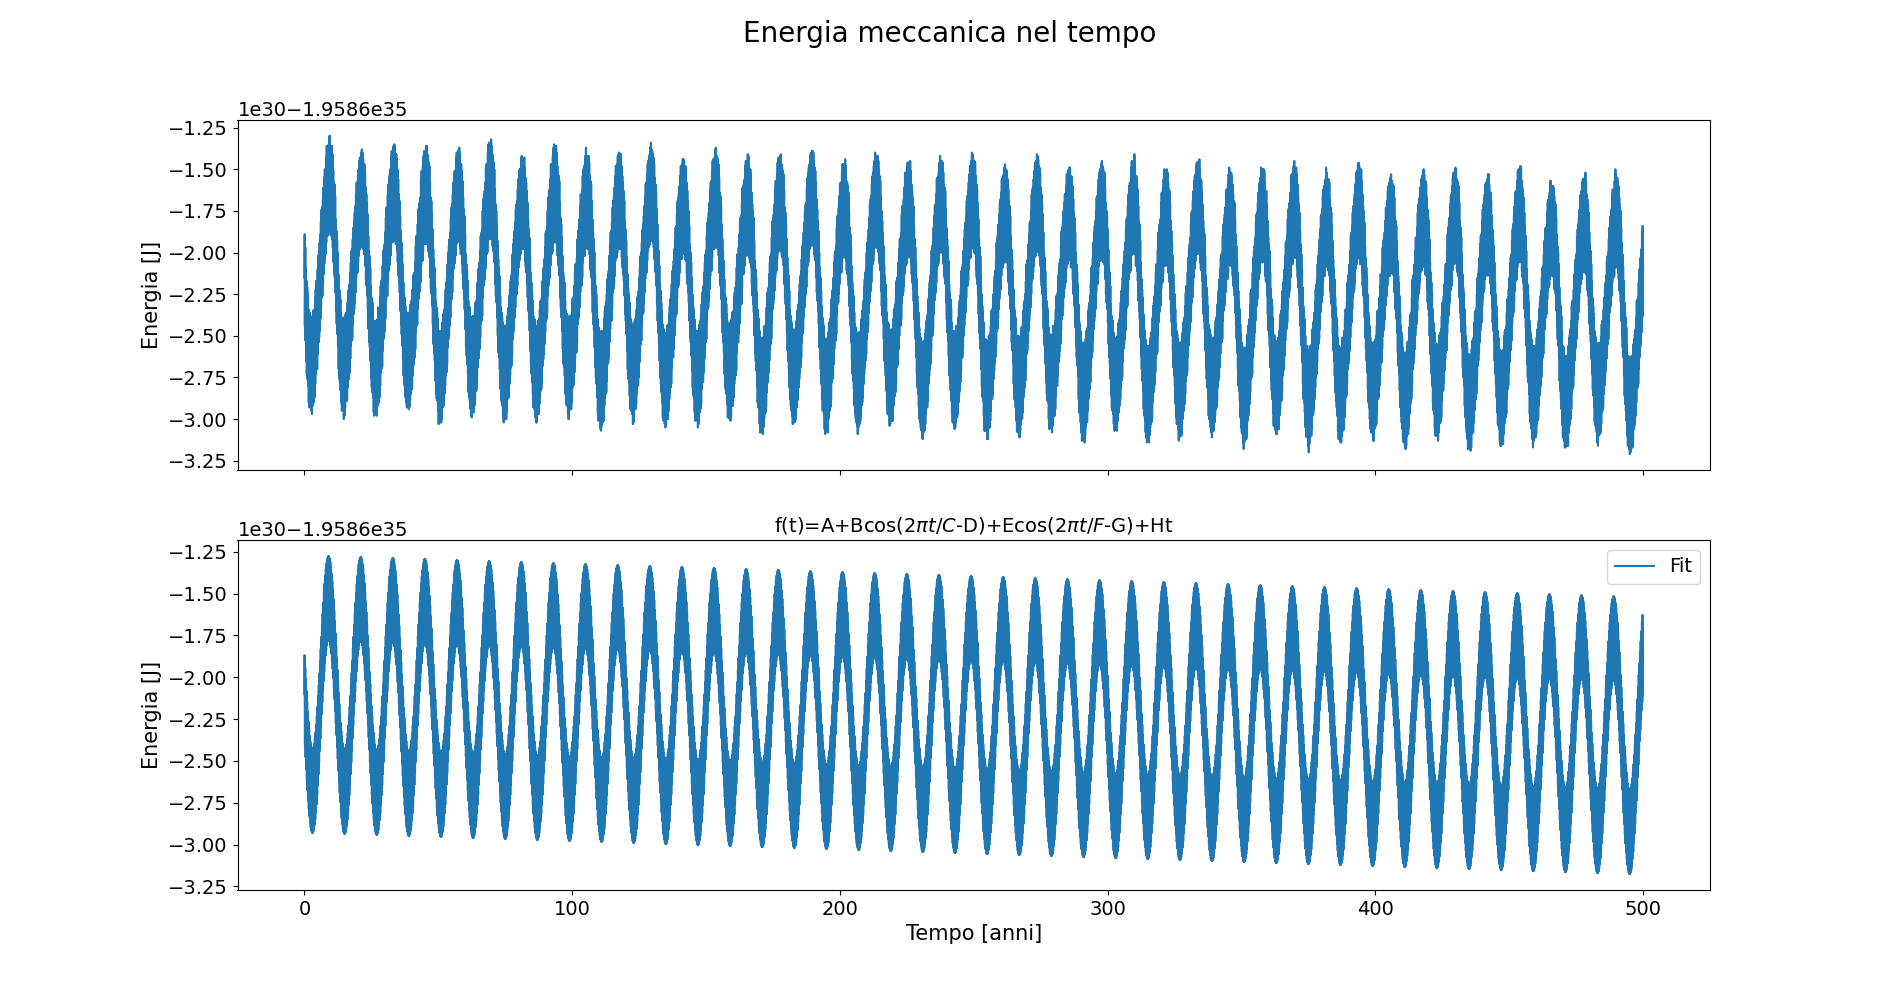
\includegraphics[width=\textwidth]{4_energia/peak/mec_500_2.png}\\
                \label{cfr::E6T}    
            \end{figure}  
            T portante= $ 12.000008934962754 \pm 0.10447251253008041$ anni\\
            Pendenza decrescita= -5e+26 Joule
        \end{frame}
        \begin{frame}{Andamenti nel tempo}
            \begin{figure}
                \centering
                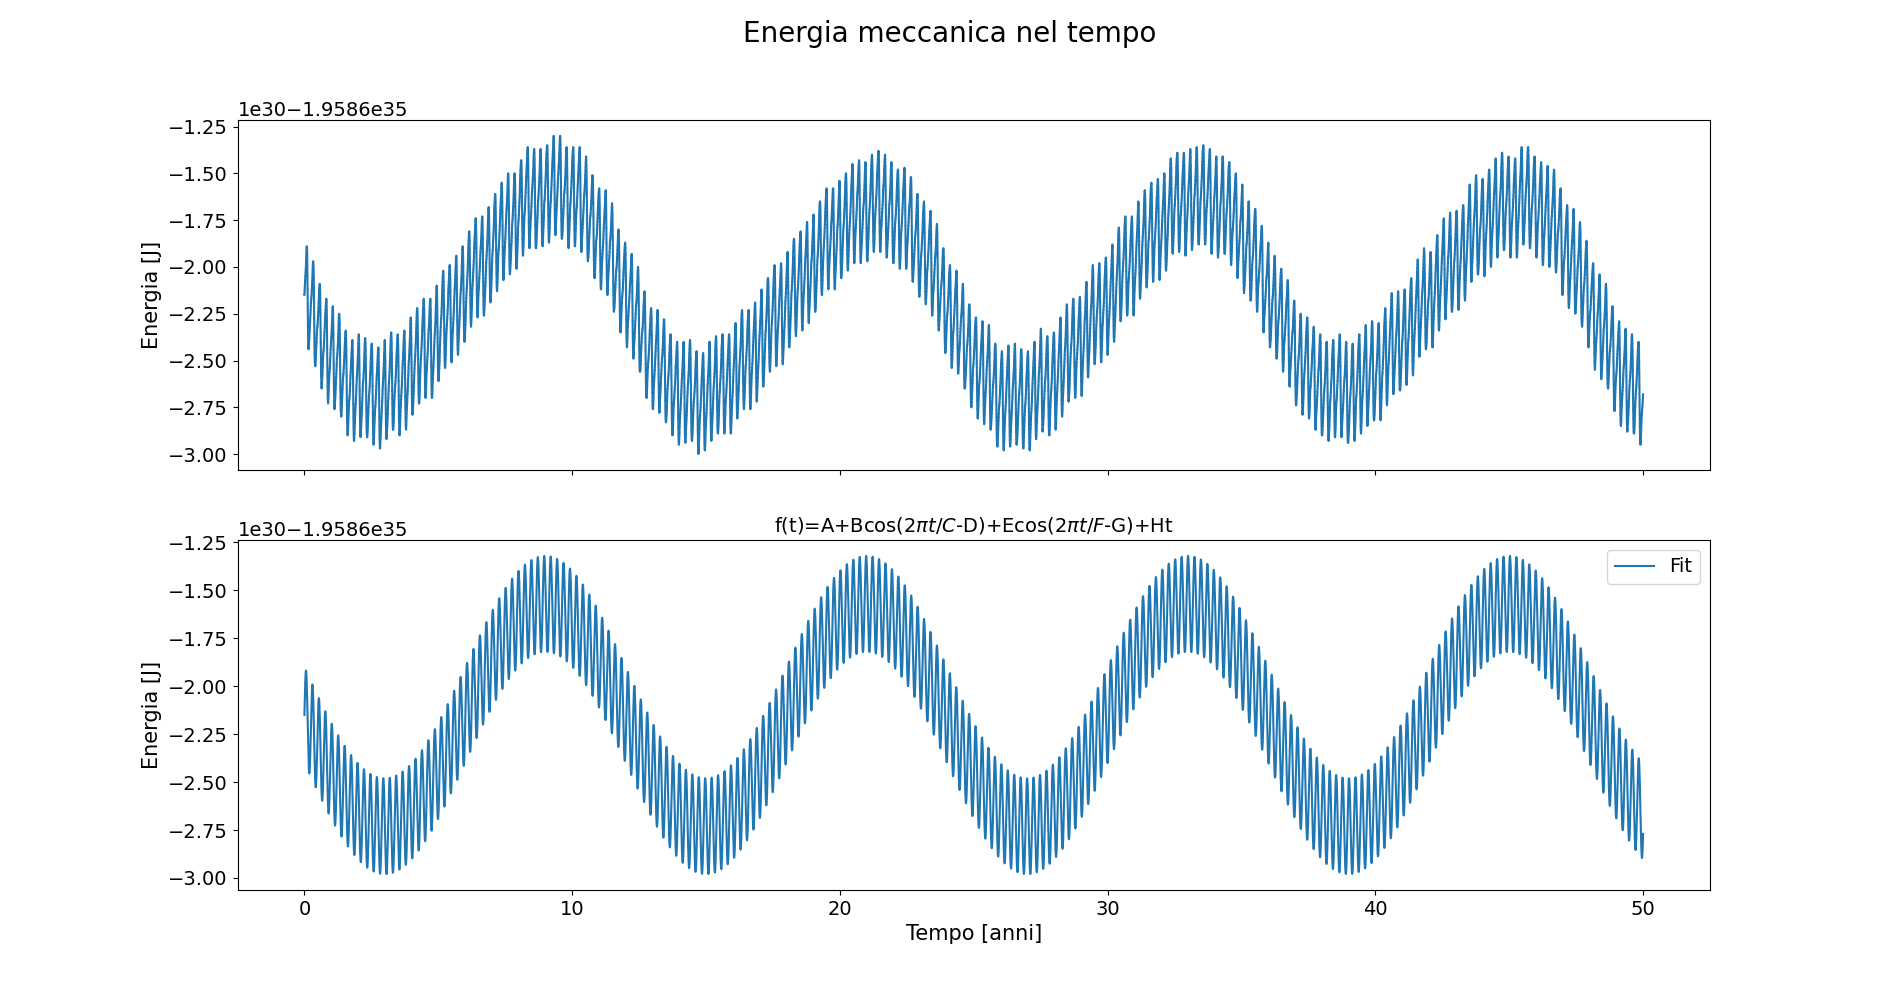
\includegraphics[width=\textwidth]{4_energia/peak/mec_50_1.png}\\
                \label{cfr::E6T}    
            \end{figure}  
            T modulante= $87.84482197184609 \pm 0.03564632637201194$ giorni\\
        \end{frame}

        \begin{frame}{Possibile spigazione}
            \begin{columns}
                \column{.5\textwidth}
                    \begin{itemize}
                        \item Influenza del moto di Giove
                        \item Il Sole non rimane fisso nell'origine
                        \item[$\Rightarrow$] Differenze tra due tratti dell'orbita di Giove
                    \end{itemize}
                \column{.5\textwidth}
                    \centering        
                    \includegraphics[width=5cm, height=3.75cm]{4_energia/peak/.jpg}\\
                    %qui grafico moto di giove 
                    \label{cfr::eme}      
            \end{columns}
            \begin{figure}
                \centering
                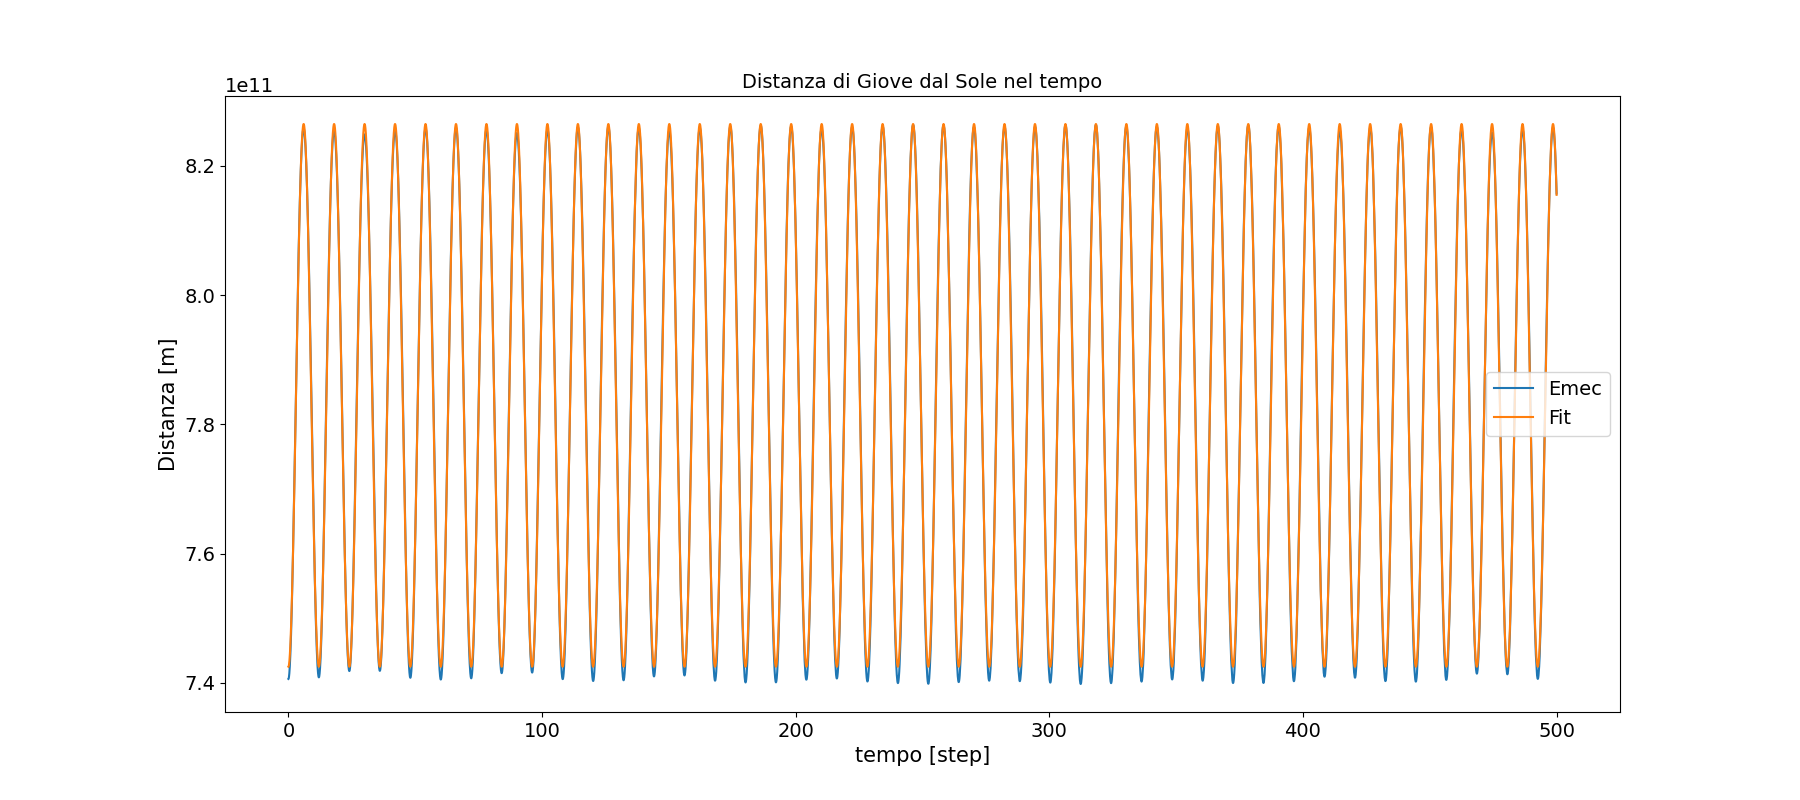
\includegraphics[height=3.75cm]{4_energia/peak/giove_fit.png}\\
            \end{figure}
        \end{frame}

        \begin{frame}{Verifica}
            \begin{columns}
                \column{.5\textwidth}
                    Simulazione con Sole fisso nell'origine del sistema di riferimento\\
                    OSS: Potrebbe spiegare anche i grafici precedenti\\
                    \vspace{1cm}
                    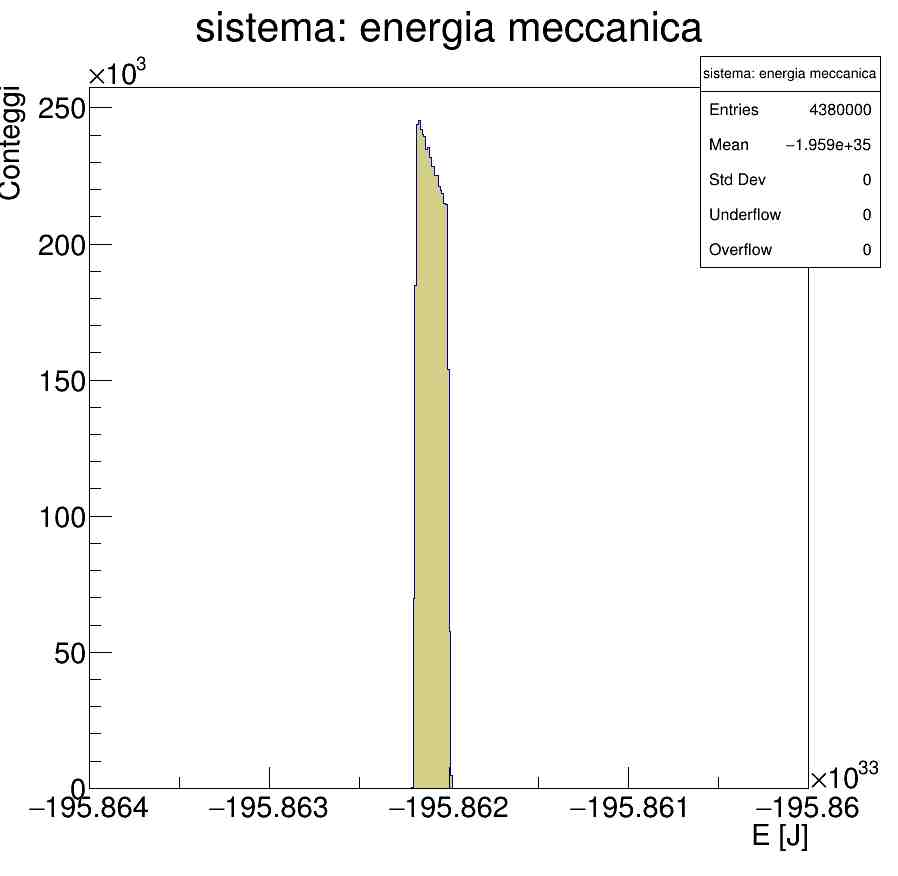
\includegraphics[width=5cm,height=3.75cm]{4_energia/peak/sf_E.jpg}\\
                \column{.5\textwidth}
                    \centering        
                    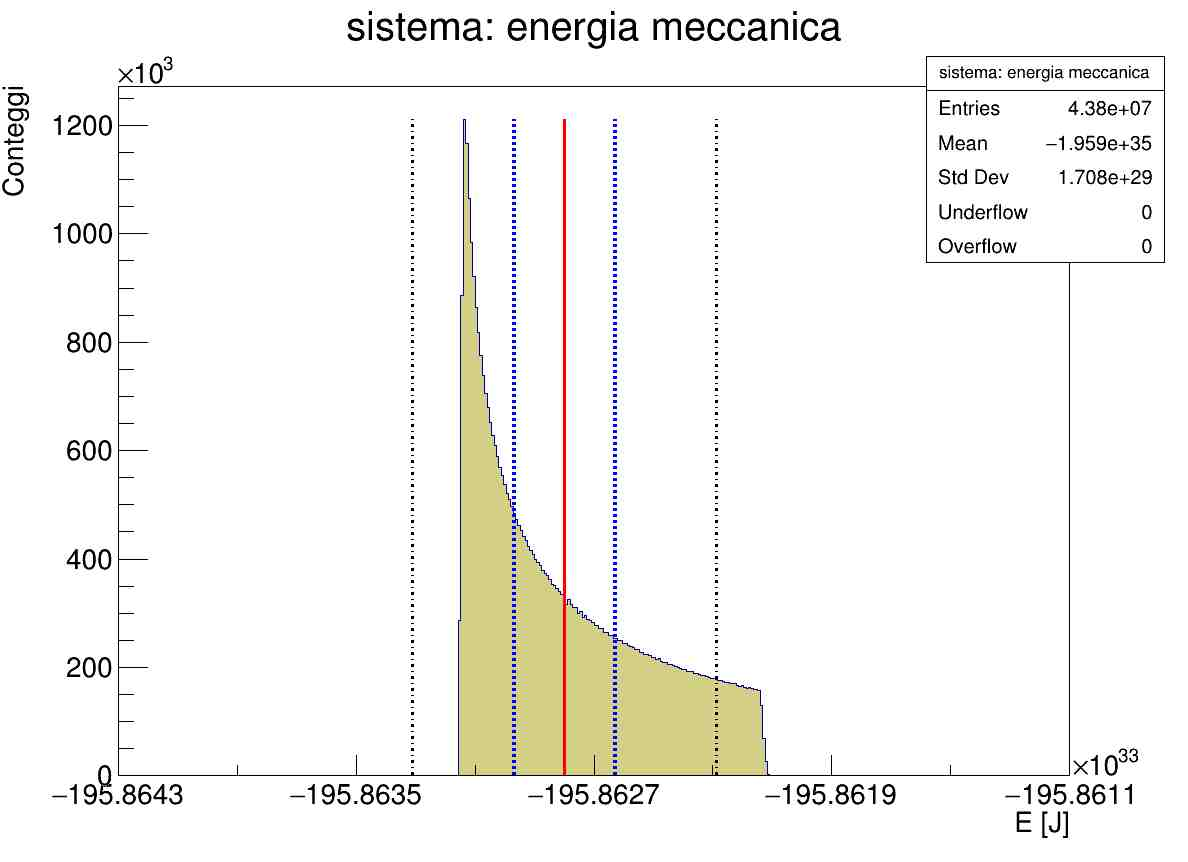
\includegraphics[width=5cm,height=3.75cm]{4_energia/peak/5000.jpg}\\
                    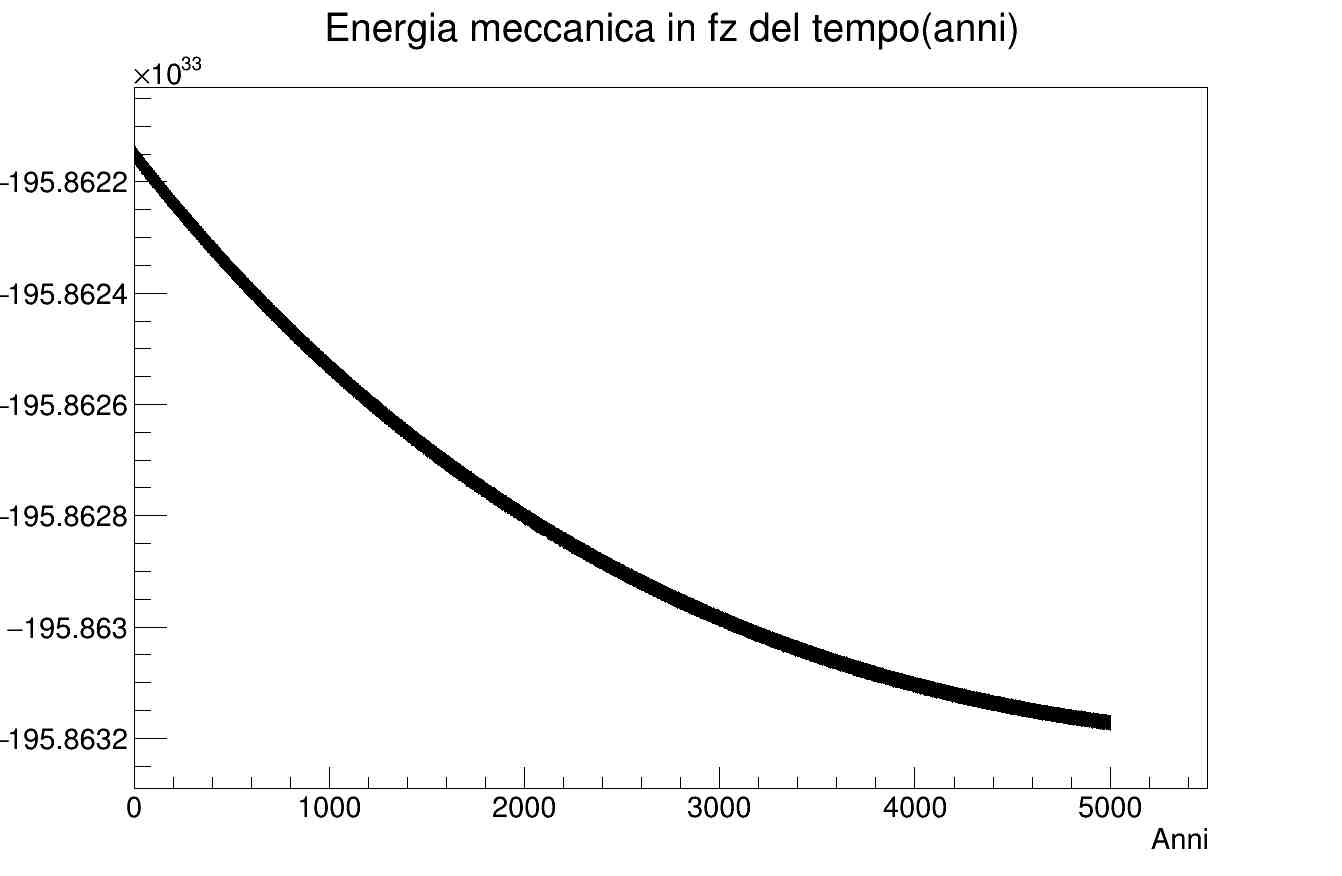
\includegraphics[width=5cm,height=3.75cm]{4_energia/peak/5000_tempo.jpg}
                    \label{cfr::eme}      
            \end{columns}
        \end{frame}
